\documentclass[11pt,a4paper]{article}

% Packages
\usepackage[utf8]{inputenc}
\usepackage[spanish, es-tabla]{babel}
\usepackage{caption}
\usepackage{listings}
\usepackage{adjustbox}
\usepackage{enumitem}
\usepackage{boldline}
\usepackage{amssymb, amsmath}
\usepackage{amsthm}
\usepackage[margin=1in]{geometry}
\usepackage{xcolor}
\usepackage{soul}
\usepackage{hyperref}

% Meta
\date{\today}

% Custom
\providecommand{\abs}[1]{\lvert#1\rvert}
\setlength\parindent{0pt}
\definecolor{Light}{gray}{.90}
\newcommand\ddfrac[2]{\frac{\displaystyle #1}{\displaystyle #2}}
% Primera derivada parcial: \pder[f]{x}
\newcommand{\pder}[2][]{\frac{\partial#1}{\partial#2}}

\begin{document}
\begin{titlepage}
\begin{center}

\vspace*{.06\textheight}
{\scshape\LARGE Universidad De Granada\par}\vspace{1.5cm} % University name
\textsc{\Large Apredizaje Automático}\\[0.5cm] % Thesis type

\rule{\textwidth}{0.4mm} \\[0.4cm] % Horizontal line
{\huge \bfseries Proyecto Final\par}\vspace{0.4cm} % Thesis title

\rule{\textwidth}{0.4mm} \\[11.5cm] % Horizontal line
 {\Large Pedro Bonilla Nadal\\Antonio Martín Ruiz}\\[1cm]

 {\today}

\vfill
\end{center}
\end{titlepage}

\setcounter{tocdepth}{2}
\tableofcontents
\newpage



\section{Comprensión del problema a resolver }

Este dataset contiene datos de la oficina del censo\cite{census} relativos a censos de 1995, obtenidos del repositorio UCI de bases de datos \cite{uci}. Un total de 48842 personas han sido encuestadas para este censo. De estas personas tenemos una serie de variables con información de carácter socioeconómico. En particular:
\begin{itemize}
\item Tenemos 6 variables de tipo numérico u ordinal, con valores en rangos distintos.
\item 8 variables de tipo categórico.
\item Una variable de clase que toma como valores $<50$K y $>50$k.
\item Es un problema de clasificación, ya que no tenemos información para hacer una regresión sobre la ganancia.
\end{itemize}

El código utilizado para la resolución de la práctica se encuentra en el archivo \texttt{main.py}.  Del mismo modo, los datos limpiados se encuentran en el archivo \texttt{adults.data} y su información relativa procesada en el archivo \texttt{adult.names}.


\section{ División y codificación de los datos}

A la hora de obtener los datos en el respositorio se encuentran tres archivos: \texttt{adult.data},  \texttt{adult.test} y \texttt{adult.names}. Estos datos fueron procesados en el año 1996. Nosotros realizamos una operación de formato de los datos para ajustarlos a convenciones más recientes.

\begin{itemize}
\item Cambiamos la variable de clase por valores categóricos 0 para $<50$K y 1 para $>50$K.
\item Eliminamos el espaciado después de la coma para facilitar la lectura por parte de librerías actuales.
\item Añadimos el flag \texttt{@attribute} a la lista de atributos provista en \texttt{adult.names}.
\end{itemize}

Utilizaremos la división train/test que viene establecida por el propio dataset. La proporción de clases es parecida en ambos conjuntos y la cantidad de datos en el training establecido es la suficiente para el aprendizaje. Es por ello que no modificamos esta partición. Además, a la hora de validar la selección de hiperparámetros utilizaremos la técnica cross validation, para la cual dividiremos el conjunto de training en 5 subconjuntos. Se utilizará para esta la función \texttt{cross\_validate}\cite{cv}.\\

Como ultimo detalle de codificación de los datos durante la parte de preprocesado aplicamos la codificación sugerida por scikit-learn mediante \texttt{dummy\_variables}. Mediante este proceso se transforman las variables categóricas en numéricas dale un valor natural diferente a la variable para cada tipo de valor que tomara anteriormente.

\section{Preprocesado}

Mostraremos a continuación las siguientes técnicas de preprocesado realizadas. Justificaremos individualmente su uso.

\begin{itemize}

	\item \underline{Normalización de las variables}. Realizaremos una normalización de los datos, para evitar que su escala afecte a la relevancia de estos. Para ello usaremos la función \texttt{StandardScaler}\cite{standardscaler} provista en la librería \texttt{sklearn}.
		\item \underline{Valoración del interés de la variables}. Para esto vamos a realizar dos técnicas:
	
	\begin{itemize}
	\item[-] El conjunto de datos presenta 105 columnas. Por ello vamos a intentar reducir aquellas que presenten poca o ningúna información haciendo un análisis por varianza, y eliminando aquellas columnas cuya varianza sea inferior a 0.1. Esto lo realizaremos con el algoritmo \texttt{varianceThreshold}\cite{einstein}.
			
\begin{table}[h]
\begin{center}
\begin{tabular}{|l|c|}
\hline
 Proceso & Dimensionalidad Resultante \\ \hline
 \texttt{Dummy\_Variables} &  105\\
\texttt{varianceThreshold} &57 \\\hline
\end{tabular}
\end{center}
\caption{Dimensionalidad de la muestra tras cada proceso.}
	\end{table}



Podemos observar como tenemos una gran cantidad de variables que aportan poca o ninguna información. Observando la muestra atentamente veremos que se debe a variables como \texttt{nacionality}, que tras ser codificadas como dummy variables quedan como columnas nacionalidades con muy pocos positivos. Esto es negativo porque da pie a que algunos algoritmos (en particular los basados en árboles) sobreajusten a esta submuestra en particular. \\

\item Además realizamos un estudio \texttt{PCA} con el objetivo de avergiguar cuales son las columnas que mejor explican la variabilidad de la base de datos. Para ello ejecutamos un predictor \texttt{PCA}, así como \underline{seleccionar las variables principales}. Este nos devuelve una estimación de la variabilidad que explica cada variable, obteniendo como resultado:
\begin{figure}[h]
{\center
\texttt{
[4.49573987e+00 2.94835042e+00 2.37099181e+00 \\
\ 2.01320755e+00 1.76975896e+00 1.75675195e+00 \\
\ 1.68179310e+00 1.42475478e+00 1.38339986e+00\\
\ 1.32481406e+00 1.28634456e+00 1.24730223e+00\\
\ 1.19496365e+00 1.17428828e+00 1.15682951e+00\\
\ 1.13753027e+00 1.12467327e+00 1.11347522e+00\\
\ 1.09735994e+00 1.07570368e+00 1.07225031e+00\\
\ 1.06723994e+00 1.03858652e+00 1.02811739e+00\\
\ 1.02497765e+00 1.01754201e+00 1.01319671e+00\\
\ 1.00978578e+00 1.00228665e+00 9.92216208e-01\\
\ 9.86143567e-01 9.81570539e-01 9.65009215e-01\\
\ 9.52551640e-01 9.38447568e-01 9.16648964e-01\\
\ 8.97850717e-01 8.77922999e-01 8.31440082e-01\\
\ 7.68450694e-01 7.55866947e-01 7.14349376e-01\\
\ 6.89593020e-01 6.14759178e-01 5.64426417e-01\\
\ 5.22746091e-01 4.35534961e-01 4.01351472e-01\\
\ 7.00012064e-02 4.35859769e-02 2.11241135e-02\\
\ 5.56548322e-03 1.52954845e-03 1.03141699e-03\\
\ 1.72725144e-05 1.17471416e-31 9.16296960e-33]\\}
}
\caption{Resultado algoritmo PCA}
\end{figure}

Como podemos observar tenemos una diferencia significativa con respecto a las dos últimas variables, por lo que decidimos desestimarlas. Con esto obtenemos loas resultados.

		
\begin{table}[h]
\begin{center}
\begin{tabular}{|l|c|}
\hline
 Proceso & Dimensionalidad Resultante \\ \hline
  \texttt{varianceThreshold} &57 \\
\texttt{PCA} &55 \\\hline
\end{tabular}
\end{center}
\caption{Dimensionalidad de la muestra tras cada proceso.}
	\end{table}

\end{itemize}
\newpage
\item  \underline{Polynomial Freatures}. Con especial interés en el caso lineal, el uso de variaciónes polinómicas de los datos puede ser util para permitir aproximaciones a clases de funciones nuevas. Probaremos variación cuadrática sobre las variables numéricas cuando realizemos un ajuste lineal. Para Random Forest no lo consideramos necesario por la ya conocida complejidad de los arboles, y para SVM utilizaremos variaciones de kernel. \\
	
	\item \underline{Valoración de las variables de interés}. Para realizar un estudio de las variables de interés. Este ya lo hemos visto mostrado en 
	\item \underline{Datos incompletos y valores perdidos}. En relación a los valores perdidos encontramos en tres variables de tipo categórico.\\
	
\begin{table}[h]
\begin{center}
\begin{tabular}{|l|ll|}
\hline
Variable& Valores distintos & Valores Perdidos\\ \hline
\texttt{workclass} & 9 & 2799\\
\texttt{occupation} & 15 & 2809\\
\texttt{native-country} & 42 & 857\\\hline
\end{tabular}
\end{center}
\caption{Representación de valores perdidos.}
	\end{table}
	
	Realizamos la sustitución de estos datos mediante la función \texttt{replace\_lost\_categorical\_values}. En esta, para cada columna, calculamos su distribución de probabilidad, esto es, sumamos las ocurrencias de cada categoría y dividimos entre el total de valores con valores no perdidos. Obtenemos así la probabilidad de cada categoría. A continuación calculamos las probabilidades acumuladas sumando para categoría su probablidad y la de todas las anteriores. Para cada dato perdido generamos un número aleatorio mediante una distribución uniforme en el intervalo $[0,1]$. La clase por la que el valor perdido será sustituida será la de cuyo intervalo contenga al valor generado, siendo el intervalo de cada clase el comprendido entre la probabilidad acumulada de la anterior y su probabilidad acumulada (incluyendo en cada uno su extremo inferior, pero no su extremo superior).
	
	\item \underline{Datos inconsistentes}. No encontramos datos inconsistentes.
	\item \underline{Balanceo de clases}. Nos encontramos ante una situación con un desbalanceo notable. Sin embargo, dada la cantidad de datos provista por la base de datos creemos que no es necesario realizar modificaciones de los datos ni en el conjunto de train ni en el de test.
\end{itemize}

\section{ Métricas }

Hemos decidido considerar, en este contexto de clasificación, dos funciones con objetivo de medir el error, ambas halladas en \cite{met}.
\begin{itemize}
	\item \emph{accuracy}. Decidimos utilizar esta medida como principal por su simplicidad y expresividad. Esta métrica nos propocionará una idea general de la bondad de nuestro modelo en un caso general, así como nos permitirá comparar, por ejemplo, con el clasificador modal. 
	\item \emph{f1-score}. Al estar en un modelo de clases desbalanceadas, consideramos que debiamos utilizar además una métrica que penara comportamientos de 'asignación modal'. La medida $F_1$ se define como\cite{f1}
	$${\displaystyle F_{1}={\frac {2}{\mathrm {recall} ^{-1}+\mathrm {precision} ^{-1}}}=2\cdot {\frac {\mathrm {precision} \cdot \mathrm {recall} }{\mathrm {precision} +\mathrm {recall} }}}.$$
	
	donde precisión es (en términos de clase positiva/negativa) el número de verdaderos positivos entre los positivos escogidos, y recall es el número de positivos escogidos entre los positivos totales. En este caso la medida que mostramos es la media obtenida de las f1-score obtenidas de considerar cada una de las clases como la positiva.
\end{itemize}
\section{ Modelos Considerados }
TODO: añadir las funciones y links a estas en la bibliografía.
\subsection{ Modelo lineal }
	
	Como modelo lineal, dado que estamos en clasificación, podemos escoger de los modelos explicados en clase entre Regresión Logística y  PLA. Decidimos utilizar regresión logística por una serie de motivos.
	
	\begin{itemize}
	\item Al estar en un dataset que proviene de un censo sucede que podemos encontrar una gran cantidad de outliers y datos algo ruidosos. Esto hará que el perceptron sea contraindicado, dado que dificilmente podremos conseguir convergencia de este debido al ruido, y en el caso de que uno de estos elementos ruidosos sea además un outlier podría variar notable (e indebidamente) el plano clasificador.
	\item Nos resulta interesante el hecho de que podamos obtener la confianza de una predicción y no solo la predicción.
\end{itemize}

Para el uso de la regresión logistica haremos uso de la función de sklearn. 

\subsection{Random Forest}

El principal objetivo que justifica la aplicación de esta técnica generar un modelo complejo que represente con mucha precisión el conjunto de entrenamiento. Esto nos permitirá su comparación con otros modelos más sencillos que produzcan un ajuste menos exacto de los datos. Mediante esta comparación podremos comprobar la incidencia del problema del overfitting en este caso. 

\subsection{SVM}

Consideramos que la técnica SVM-soft margin puede ser muy útil para este problema debido a que podemos fijar a placer el grado de compromiso entre busqueda del plano óptimo y la tolerancia al ruido, ambas cosas resultando de mucha utilidad a la hora de trabajar con datos potencialmente ruidosos.\\

Otro motivo para decidir ajustar este modelo, aunque de carácter menos importante, es la curiosidad suscitada por este modelo durante el desarrollo teórico de la asignatura. 

\section{ Técnica de Ajuste para el Modelo Lineal}
Para este conjunto utilizaremos dos técinas de ajuste, ambas definidas como variaciones especializadas sobre el algoritmo SGD.:
\begin{itemize}
	\item \texttt{lbfgs}. Utiliza una variación del método Newton visto en el bonus de la práctica 1 que en lugar de la matriz Hessiana utiliza una aproximación a esta. Es eficiente en comparación con el método de newton estandard y se podría definir como una variación del gradiente descendente estocástico. Como desventajas tiene que se podría acercar a puntos críticos que no fuese mínimos. Esta técnica no admite regularización \texttt{l1}.
	\item \texttt{liblinear}. Es el ganador ICML 2008 large-scale learning challenge. Lo utilizamos para probar las regularizaciónes dado que funciona tanto con \texttt{l1} como con \texttt{l2}.
	
	Liblinear utiliza técnicas de descenso coordinado\cite{CD} donde minimizamos la función en torno a cada eje, resolviendo un problema de minimización unidimensional en bucle. 
\end{itemize}

Estas dos técnicas se pueden entender como variaciones del gradiente descendiente estocastico en esecia, dado que surgen de su filosofía de realizar aproximaciones sucesivas al mínimo. Pese a ello se debe comprender que se parecen en poco más que filosofía. Son técnicas mucho más eficientes que el algoritmo de la pseudoinversa, cosa que nos puede resultar interesante, aunque trabajamos con un dataset que no es particularmente grande. Las compararemos y comentaremos sus resultados  en la sección de hiperparámetros y selección del modelo, pero elegiremos lbfgs dado que para el tamaño de nuestro dataset no es relevante la mejora en eficiencia de \texttt{liblinear} y \texttt{lbfgs} consigue un resultado ligeramente mejor.


\section{Hiperparámetros y selección del modelo}
 En esta sección estudiaremos la aplicación de las técnicas especificando claramente qué algoritmos se usan en la estimación de los parámetros, los hiperparámetros y el error de generalización.\\
 
 
 El primer modelo que presentamos es el modelo lineal. Este fue el primer modelo ajustado y de su ajuste aprovechamos conocimiento para el ajuste de los otro modelos. 
 
\subsection{Modelo Lineal}
Como hiperparámetro vamos a considerar la prueba de las dos distintas técnicas de ajuste, las dos técnicas de regularización, así como la fuerza de regularización. También consideraremos una muestra con variables lineales y otra con variables polinómicas. \\



\begin{itemize}
\item \underline{Variables polinómicas}: Como primera aproximación al problema estidiamos, con un estimador base, la mejora supuesta al aumentar la dimensionalidad del dataset al incluir variables polinómicas. Con esto pretendemos ver si el modelo lineal es suficiente para explicar la variabilidad de la muestra. Obtenemos como resultados las siguientes estimaciones\footnote{Estimaciones de error con  5Fold-Cross-Validation.}:

\begin{table}[h]
\begin{center}
\begin{tabular}{|l|c|c|}
\hline
	Grado & Accuracy & F1 \\ \hline
1 & 0.85061 & 0.78141 \\
2 & 0.85061 & 0.78141  \\\hline
\end{tabular}
\caption{Resultados ajustes con variables polinómicas.}

\end{center}
\end{table}

Lo primero que observamos es que, debido a la cantidad y dimensionalidad de los datos sucede que para generar una base de datos con cobinaciones cúbicas creamos un conjunto de 8.30 GB que no somos capaces de alojar en la RAM del procesador. Es por eso que, por las limitaciónes técnicas que poseemos no consideramos más grado\footnote{En el código entregado no adjuntamos esta ejecución para evitar entregar un código que no funcione de principio a fin, lo que provocaría la descalificación de la práctica}. De todos modos esta limitación no nos afecta pues:
\begin{itemize}
	\item Estaríamos en un caso claro de Maldición de la Dimensionalidad\cite{maldim} a pesar de haber realizado ya una reducción de dimenisonalidad tanto por \texttt{varianceThreshold} como por \texttt{PCA}.
	\item Podemos ver que se mantiene invariable la estimación del error invariante. Esto es resultado a que el modelo lineal ya se ajusta perfectamente a la variabilidad de los datos. 
\end{itemize}

Es por esto que decidimos \underline{no aplicar esta técnica}.
\item \underline{Regularización}. Empezamos considerando que regularización debemos usar. Barajamos como opciones regularización \texttt{l1} y regularización \texttt{l2}. Durante el desarrollo de la asignatura hemos aprendido que cada una de estas penaliza de forma distinta. En particular:
  \begin{itemize}
  \item \texttt{l1}: penaliza si habia variables que podrían no ser relevantes. Esta es mejor en caso de alta dimensionalidad.
  \item \texttt{l2}: penaliza que todas estas sean relevantes. Esta es mejor en casos de datos con alta cantidad de outliers.
  \end{itemize}

  Utilizando conocimiento del mundo en el que vivimos es fácil imaginar que en un censo económico hay muchos outliers, que consistirán en la gente más privilegiada. Sin embargo no utilizaremos esta información y usaremos datos puramente analíticos. Podemos considerar dos casos:
  \begin{itemize}
  \item \emph{Outliers de variables categóricas}: Estos han sido gestionados ya, debido al one-hot-encoding realizado durante la codificación del dataset, así como el filtro de varianza, ha hecho que todas las categorías sin un número significativo de personas incluido sean desestimadas.
  \item \emph{Outliers de variables ordinales}: Para el estudio de este examinamos una a una las variables, imprimiendo el gráfico[\ref{fig:outliers}].Podemos ver que tenemos una gran cantidad de outliers. En particular tenemos distribuciones de cola larga o \emph{Heavy Tail} como son conocidas en el mundo de la estadística. Estas distribuciones son aquellas en las cuales, pese a estar la mayoría de los valores agregados en un espacio pequeño del dominio.\\

    Por otro lado podemos ver que después del preprocesado, hemos descartado una gran cantidad de variables (casi la mitad) y hemos estudiado con \texttt{PCA} que el resto de variables consideradas aportan información para explicar la variabilidad de la muestra. Es por esto que no consideramos que la regularización \texttt{l1} pueda aportar mucho al modelo.\newpage

    \begin{figure}[h!]    
      \centering
      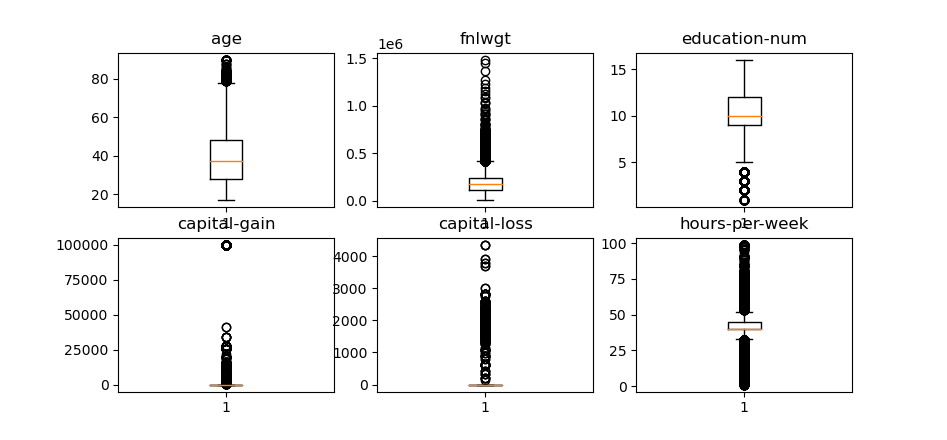
\includegraphics[width=\textwidth]{./figures/outliers.png}
      \caption{Representación de las variables ordinales. }
      \label{fig:outliers}
    \end{figure}

  \end{itemize}

Debido a esto decidimos usar regularización \texttt{l2}. 

\item \underline{Técnica de ajuste}: No tenemos ningún argumento en contra o a favor de la técnica de ajuste elegida. Probaremos ambas y eligiremos la que mejor error bondad de ajuste aproxime. Tras las pruebas obtenemos que la mejor técnica el \texttt{liblinear}, aunque las diferencias con mínimas.

\item \underline{Fuerza Regularización}:   Para seleccionar la fuerza de ajuste realizaremos una representación de esta, con el objetivo de estimar una cantidad óptima. Obtenemos como resultado:
    \begin{figure}[h!]
      \label{figure:regularization}
      \centering
      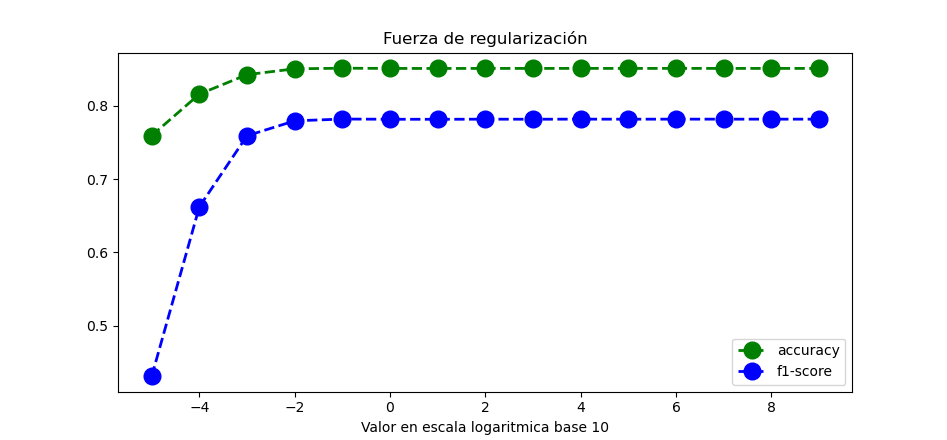
\includegraphics[width=\textwidth]{./figures/regularizacion_rl.png}
      \caption{Relación de las métricas de error con la regularización.}
    \end{figure}

Podemos ver que en valores muy pequeños de va fuerza de regularización, obtenemos un peor resultado, y que se estabiliza a partir de valores mayores. Elegimos como mejor resultado tras realizar una ingeniería de parámetros un poco más exhaustiva, elegimos como valor de la fuerza de regularización 2.\\
\end{itemize}


Así obtenemos que el mejor ajuste es:

{\begin{center}
    \texttt{LR( penalty='l2', random\_state=0, solver='liblinear', C=1.9)}
  \end{center}}

Obtenemos los resultados:

\begin{table}[h]
\begin{center}
\begin{tabular}{|l|c|c|}
\hline
  Error & Accuracy & F1-score \\ \hline
  $E_{in}$ & 0.85132 & 0.78230 \\
  $E_{test}$ & 0.84976 & 0.77027  \\
  $E_{cv}$ &0.85064 & 0.78150  \\\hline
\end{tabular}
\caption{Resultados ajustes con variables polinómicas.}

\end{center}
\end{table}

\subsection{Random forest}

A partir del modelo por defecto que proporciona scikit-learn modificaremos tres parámetros para obtener el resultado final

\begin{itemize}
\item \underline{Número de estimadores}. Viene dado por el parámetro \texttt{n\_estimators}. El número por defecto es 100. Procedemos ampliando este número hasta que dejan de producirse mejoras significativas. En las gráficas vemos cómo evoluciona la puntuación en la predicción dentro de test y en cross validation. Comenzamos con un número pequeño de estimadores y comprobamos que la predicción dentro del test sube hasta llegar a los 100 iteradores, donde ya es prácticamente perfecta. En cross validation observamos que la subida es equivalente hasta los 100 estimadores, pero a partir de aquí la predicción baja. Comprobamos un repunte en 400 estimadores y a partir de este punto podemos considerar que empieza a crecer el overfitting. Obtenemos entonces que el número óptimo es el de 400 estimadores.

    \begin{figure}[h!]
      \label{figure:rf_estimadores_ein}
      \centering
      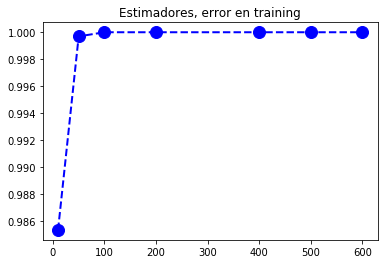
\includegraphics[width=\textwidth, scale = 0.3]{./figures/rf_estimadores_ein.png}
      \caption{Evolución d ela predicción en train según número de estimadores.}
    \end{figure}


    \begin{figure}[h!]
      \label{figure:rf_estimadores_cv}
      \centering
      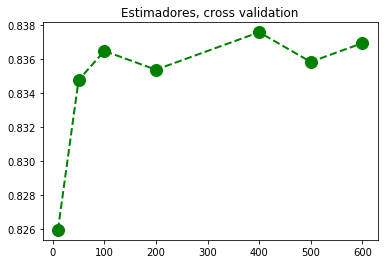
\includegraphics[width=\textwidth, scale=0.3]{./figures/rf_estimadores_cv.png}
      \caption{Evolución de la predicción en cross validation según número de estimadores.}
    \end{figure}


\item \underline{Criterio de selección}. El criterio que se aplica para obtener la calidad de las divisiones. El criterior por defecto es la impureza de Gini, pero también puede seleccionarse la ganancia de información. Puesto que esta segunda opción es la que se ha estudiado en teoría y la que produce mejores resultados, aunque con peores tiempos de ejecución, elegimos este. 
\item \underline{Profundidad máxima}. Es clave para limitar la complejidad del modelo y evitar overfitting. Por defecto la profundidad no está limitada y el árbol se amplía todo lo posible. Elegiremos limitar la profundidad de los árboles ya que obtenemos claras mejoras en clasificación. Procedemos disminuyendo este número hasta que deja de producirse una mejora en la puntuación de cross validation y empieza a empeorar el resultado. Finalmente tomamos una profundidad de 50.
\end{itemize}

Así obtenemos que el mejor ajuste es:

{\begin{center}
    \texttt{RandomForestClassifier(n\_estimators=400, criterion='entropy', max\_depth=50,)}\end{center}}
    
Obtenemos los resultados:

\begin{table}[h]
\begin{center}
\begin{tabular}{|l|c|c|}
\hline
  Error & Accuracy & F1-score \\ \hline
  $E_{in}$ & 0,9999 & 0,9999 \\
  $E_{test}$ & 0,8307 & 0,7269  \\
  $E_{cv}$ & rellenar & rellenar  \\\hline
\end{tabular}
\caption{Resultados de Random Forest.}
\end{center}
\end{table}

\newpage\hfill
\newpage
\subsection{SVM\cite{svc}}

Para el ajuste de Support Vector Machine vamos a considerar los parámetros C o fuerza de regularización y kernel. Al no tener clasificación multiclase en este problema no tiene sentido aplicar estudio de varias de las variables. También estudiaremos el parámetro max iter, aunque no lo comentaremos, procuraremos que sea lo suficientemente amplio como para obtener siempre convergencia, pero acotado para asegurar un tiempo de ejecución limitado. En general exigiremos que sea siempre inferior a 15000 iteraciones.

\begin{itemize}
\item \underline{Kernel:} Consideraremos kernel Gaussiano como viene recomendado en el guión así como lineal. No elegimos kernel polinómico debido al estudio ya realizado sobre este tema en Regresión logística.\\

Debido al éxito del modelo lineal estamos interesados en saber como se comportará un plano óptimo. Sin embargo, consideramos que la probable no existencia de un plano
  óptimo, así como la falta de variabilidad en el modelo y los habituales buenos resultados del nucleo gaussiano, hace que este se presente como una mejor alternativa. En efecto:

\begin{table}[h]
\begin{center}
\begin{tabular}{|l|c|c|}
\hline
  Nucleo & Accuracy & F1 \\ \hline
Lineal & 0.689 & 0.634 \\
Gaussiano & 0.851 & 0.781  \\\hline
\end{tabular}
\caption{Resultados ajustes con variables polinómicas.}

\end{center}
\end{table}
Por lo que escogemos nucleo Gaussiano.

\item \underline{Fuerza de regularización}: Para hacer un ajuste de esta, al igual que en modelo lineal, realizaremos un barrido de valores en escala logarítmica para detectar alguna variación grande, para posteriormente hacer una ingeniería de parámetros más fina. Obtenemos como resultado:

    \begin{figure}[h!]
      \label{figure:regularization}
      \centering
      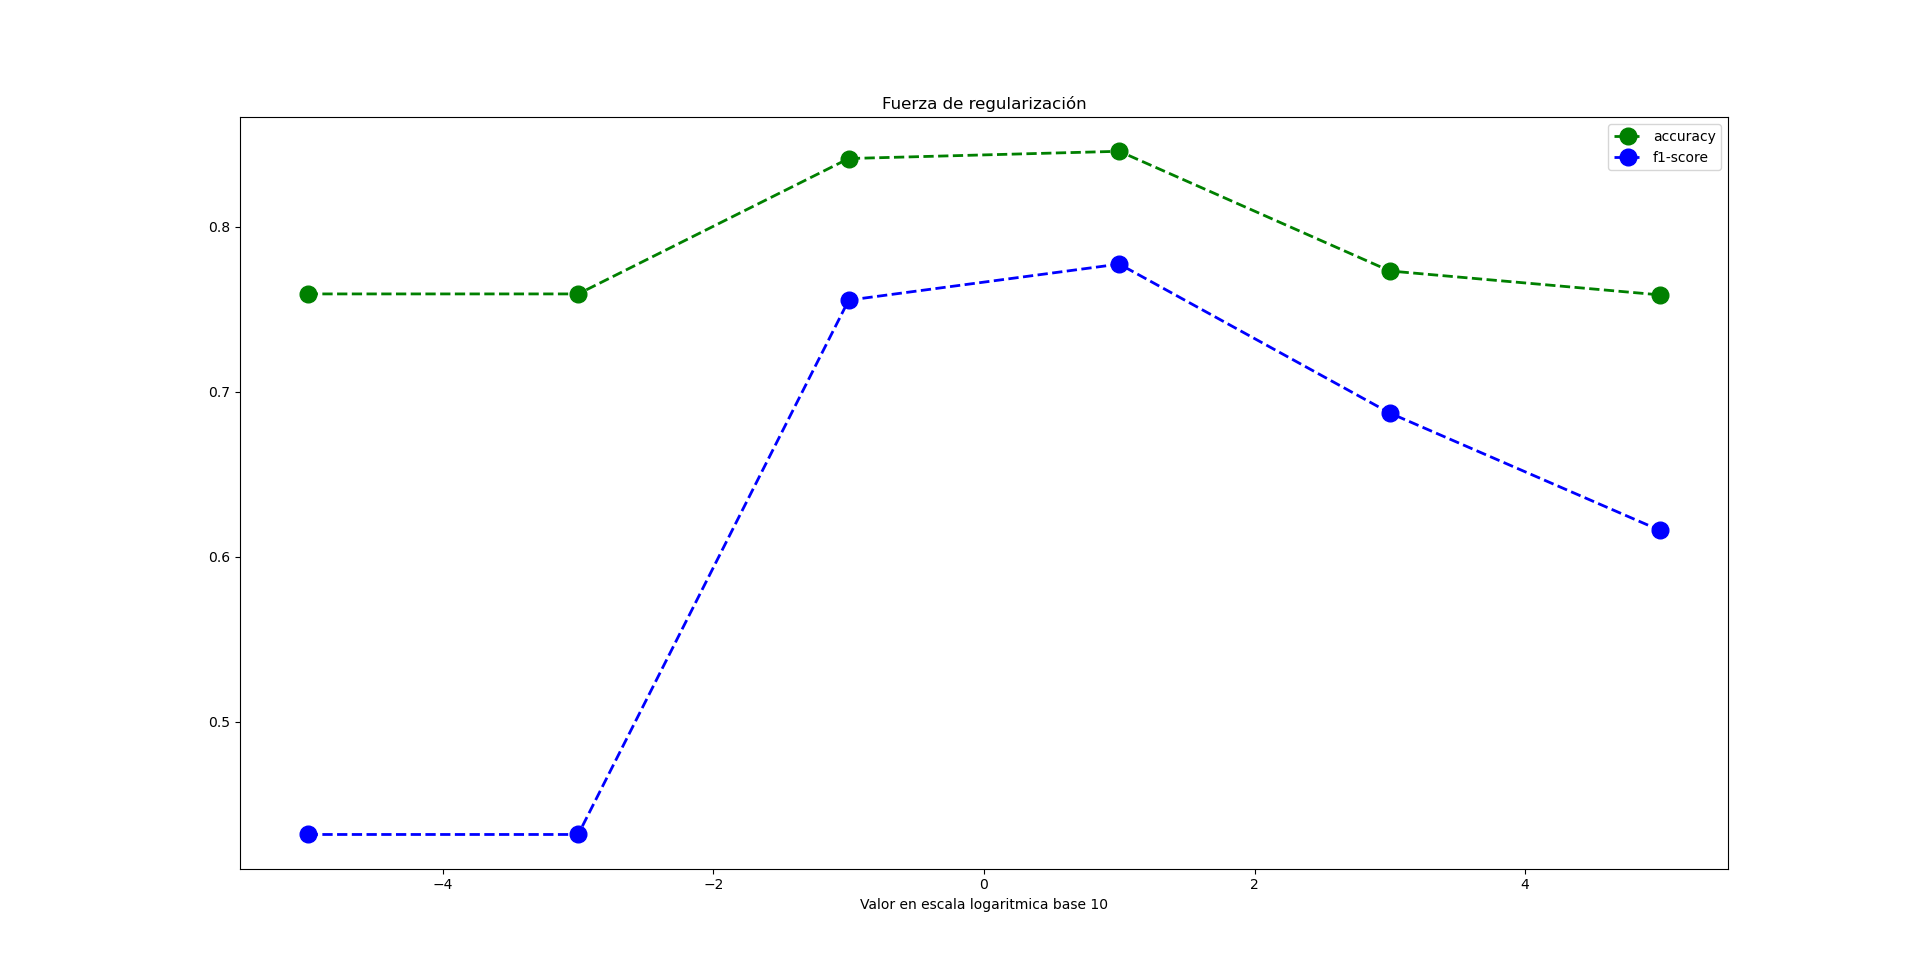
\includegraphics[width=\textwidth]{./figures/regularizacion_SVM.png}
      \caption{Progresión del error en función de la regularización.}
    \end{figure}
  
  Tras realizar un analisis exploratorio encontramos que el mejor valor es \texttt{C=2}.

\end{itemize}


Así obtenemos que el mejor ajuste es:

{\begin{center}
    \texttt{svm.SVC(max\_iter=15000, C=2, kernel=kernel)}
  \end{center}}

Obtenemos los resultados:

\begin{table}[h]
\begin{center}
\begin{tabular}{|l|c|c|}
\hline
  Error & Accuracy & F1-score \\ \hline
  $E_{in}$ & 0.87101 & 0.81114 \\
  $E_{test}$ & 0.85123 & 0.77772  \\
  $E_{cv}$ &0.85154 & 0.78153  \\\hline
\end{tabular}
\caption{Resultados ajustes con variables polinómicas.}

\end{center}
\end{table}



\section{ Error de Generalización}
\subsection{Modelo Lineal}

Tenemos un error de: Meter tabla.


\section{ Conclusiones }
Valoración de los resultados y justificación
( gráficas, métricas de error, análisis de residuos, etc )


que se ha obtenido la mejor de las posibles soluciones con la técnica elegida y la muestra dada. Argumentar en términos de los errores de ajuste y generalización. 


\newpage
\begin{thebibliography}{9}
\bibitem{census}
Página oficial de la Oficina del censo: \url{http://www.census.gov/ftp/pub/DES/www/welcome.html}.

\bibitem{uci}
Página del Centro para el Apredizaje Automático y Sistemas Inteligentes:\url{http://archive.ics.uci.edu/ml/datasets/Adult}.

\bibitem{standardscaler}
Función \texttt{StandardScaler} de la librería \texttt{sklearn}: \url{https://scikit-learn.org/stable/modules/generated/sklearn.preprocessing.StandardScaler.html}

\bibitem{cv}
Función \texttt{cross\_validate} de la librería \texttt{sklearn}:
\url{https://scikit-learn.org/stable/modules/generated/sklearn.model_selection.cross_validate.html}

\bibitem{dummy var}
Artículo donde explica el concepto de dummy variable: \url{https://en.wikipedia.org/wiki/Dummy_variable_(statistics)}

\bibitem{met}
Métricas de sklearn \url{https://scikit-learn.org/stable/modules/model_evaluation.html#balanced-accuracy-score}

\bibitem{f1}

Métrica f1-score \url{https://en.wikipedia.org/wiki/F1_score}


\bibitem{svc}
Página sklearn SVC \url{https://scikit-learn.org/stable/modules/generated/sklearn.svm.SVC.html?highlight=svc#sklearn.svm.SVC}

\bibitem{CD}
Código RL: \url{https://en.wikipedia.org/wiki/Coordinate_descent}


\bibitem{einstein} 
Uso del algoritmo \texttt{varianceThreshold}: \url{https://scikit-learn.org/stable/modules/generated/sklearn.feature_selection.VarianceThreshold.html}

\bibitem{PCA} 
Técnica de PCA: 
\url{https://scikit-learn.org/stable/modules/generated/sklearn.decomposition.PCA.html#sklearn.decomposition.PCA}

\bibitem{maldim}
Artículo donde explica el concepto de maldición de la dimensión: \url{https://en.wikipedia.org/wiki/Curse_of_dimensionality}


\end{thebibliography}





\end{document}
